\documentclass[00-livre-main.tex]{subfiles}
\begin{document}

\chapter{The Equations of a Line in Space}

Let us now think about the nature of space. Okay, that sounded goofy. I don't mean contemplating planets and nebulae and the enormity of \emph{UY Scuti}. 
So far, all of our work has been in the plane, which is supposed to represent the ideal of a flat thing which is infinite in extent and ``two-dimensional.'' Our next theater for exploration is a model for the space in which we live. Rather than having two dimensions, it has three, so we can talk about motions which are not just forward and back, and right and left, but also up and down.

Fortunately, much of the hard work we have done understanding vectors in $\R^2$ carries over quickly. There are ready analogies for point, vector, and dot product, and though the geometry of these gets more interesting, the algebra really doesn't. That will eventually be our lifeline: as the spaces we consider get more exotic, the geometries will get more complicated (and eventually almost impossible to visualize), but the corresponding algebra will always have the same level of complexity. That is why the subject is called ``Linear Algebra'' rather than ``Linear Geometry.''

Drawing pictures becomes much more challenging. One option is to study drawing and painting for a few years until representing figures from space on a plane becomes more natural. In fact, there is a strong connection between linear algebra and some of the science behind perspective drawing, which mathematicians call \emph{projective geometry}. But as that is outside the plan of our current study, we will resort to images made with software.

Again, it will take some work to get there, but we are interested in the following question:

\begin{quote}
\textbf{\large How can we clearly describe a single line in space with an equation?}
\end{quote}


\section*{Points, Vectors, and the Dot Product in $\R^3$}

Just as we worked in the plane with points and vectors (both physicist's and mathematician's vectors) by using coordinates, we can do the same for the space around us. We have the same sort of muddled trichotomy to deal with, which should feel a little less mysterious by now. Anyway, a \emph{point} in space is supposed to be a location; a \emph{(physcist's) vector} is an arrow, having direction and magnitude; and a \emph{(mathematician's) vector} is an arrow whose tail is at a special, pre-selected point called the \emph{origin} and denoted by $O$.

There are many ways to attempt to set up coordinates in space, but experience has taught us that a good way mimics the set-up from the plane. There, in the plane, we used a pair of perpendicular lines through the origin as our backdrop, which we call \emph{coordinate axes}. In space, we have more room to deal with, so instead we use three planes as reference, and we try to make them as perpendicular as we can.

How do we arrange that? The key fact we need is that when distinct planes meet, they do so along a line. 
\begin{figure}[h]
\centering
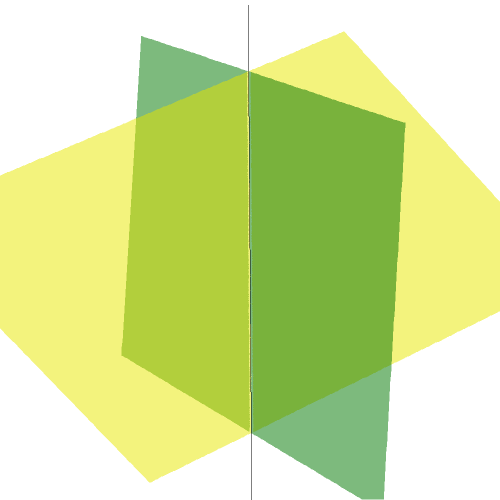
\includegraphics[width=0.3\textwidth]{images/two-planes-intersect.png}
\caption{Two planes intersect along a line.}
\label{fig:two-planes}
\end{figure}
Let's think through that a little. What does the picture look like near the intersection where two planes meet? A good way to understand it is to look ``across the intersection.'' To this end, turn the picture in front of you until the line of intersection is exactly the ``line of sight'' pointing directly away from your eye. If you do this correctly, the line should essentially vanish, by collapsing down to a single point in your vision. If you prefer, rather than imagining that you turn the picture, you can imagine moving around in space until you are in the line, and then looking in the correct direction. Either way, you should get the same image: the line of intersection collapses to a point, and the two planes under consideration collapse to lines in your vision, as you are looking at things ``edge on.''

This picture is now much simpler. We have turned the set-up of two planes which intersect along a line into a picture where two lines meet at a point. What we want is that these two lines should be perpendicular. In fact, they should mimic our usual coordinate axes picture for the plane.

So, now we are ready to set up our \emph{coordinate planes and axes} for space. First, choose a point $O$ to play the role of the origin. Then, through that point, choose three distinct planes $\p_1$, $\p_2$, and $\p_3$. Each pair of these planes meets along a line: call the intersection of plane $\p_i$ with plane $\p_j$ the line $\ell_{ij}$. So, for example, $\ell_{12}$ is the line along which plane $\p_1$ meets plane $\p_2$.

The important condition we want is this: If you look down the line $\ell_{ij}$, then the planes $\p_i$ and $p_j$ appear to be a pair of perpendicular lines. We require this to be true for each of the three lines $\ell_{ij}$ simultaneously.


\begin{figure}[h!]
\centering
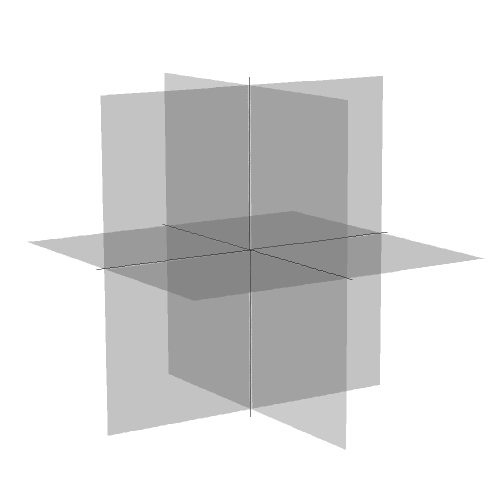
\includegraphics[width=.4\textwidth]{images/coord-planes.png}
\caption{The Coordinate Planes and Axes}
\label{fig:3d-coords}
\end{figure}

Now we are prepared to give some of these objects their traditional names. The planes $\p_1$, $\p_2$, and $\p_3$ are called the $yz$-plane, the $xz$-plane, and the $xy$-plane, respectively. The line $\ell_{12}$ is called the $z$-axis, the line $\ell_{23}$ is called the $x$ axis, and the line $\ell_{13}$ is called the $y$-axis.

Sometimes, instead of $x$, $y$, and $z$, we may use the variables $x_1$, $x_2$, and $x_3$. Then all of the names above change accordingly.

Just as in the plane, we can now introduce coordinates for points and vectors. We will just discuss how to do this for points, and you can see how to extend it to both interpretations of vectors in the same manner as before.

Given a point $P$ in space, draw a plane parallel to the $yz$-plane which passes through $P$. This plane will meet the $x$-axis in exactly one point. 
We treat the $x$-axis as a number line, so this point has associated to it a number $P_x$, which we call the \emph{$x$-coordinate of $P$}. 
Geometrically, the number $P_x$ represents the ``height'' of $P$ above the $yz$-plane. 
The words height and above are used in a relative sense, here.

Similarly, we can draw a plane parallel to the $xz$-plane which passes through $P$. This plane will intersect the number line of the $y$-axis, and we call the corresponding number $P_y$ the \emph{$y$-coordinate of $P$}. 
Finally, we can draw a plane parallel to the $xy$-plane through $P$, which will intersect the $z$-axis in a point, whose corresponding number $P_z$ is called the \emph{$z$-coordinate of $P$}. 
We then take these three numbers and bundle them together and represent the point $P$ by the ordered triple $P = (P_x, P_y, P_z)$.
Just as before, we will distinguish between points and vectors in our notation, and write vectors as vertical stacks of numbers. Here, such a stack has three parts. Motivated by our work in the plane, we make the following definition.

\begin{definition} 
A $3$-vector is a vertical stack of three real numbers, like so:
\[
v = \begin{pmatrix} v_x\\ v_y \\ v_z\end{pmatrix}.
\]
The collection of all such $3$-vectors is called \emph{$3$-space}, and written with this notation: $\R^3$.
\end{definition}

The notation $\R^3$ is often read as ``arr-three,'' and many people use that language in place of ``three-space.'' Also, most of the time we will just say ``vector'' when the context is clear. But it can be helpful to have the extra bit of information in situations where vectors of different sizes are involved.

The algebra of $3$-vectors is handled in exactly the same way as the algebra of $2$-vectors, except that there is another coordinate to track. All of the geometric connections between points, mathematician's vectors, and physicist's vectors work just as before, but there is ``more space'' to work with. Most people find visualization in three-space to be much harder than in the plane. This is completely normal, and you should expect to get used to this only if you work at it.

\begin{definition}[Algebra in $\R^3$]
Suppose that $u$ and $v$ are $3$-vectors, and that $\lambda$ and $\mu$ are scalars (real numbers). Then the \emph{linear combination of $u$ and $v$ with weights $\lambda$ and $\mu$} is defined coordinate-by-coordinate:
\[
\lambda u + \mu v = \lambda \begin{pmatrix} u_x \\ u_y \\ u_z \end{pmatrix} +
\mu \begin{pmatrix} v_x \\ v_y \\ v_z \end{pmatrix} =  
\begin{pmatrix} \lambda u_x + \mu v_x \\ \lambda  u_y + \mu v_y \\ \lambda u_z + \mu v_z \end{pmatrix} 
\]
\end{definition}

It is, of course, possible to form linear combinations of larger collections of vectors, using the corresponding number of weights. You should also notice that addition of $3$-vectors and scalar multiplication for $3$-vectors are special cases of linear combination. (How would you do this? Check this statement!) The statements of Theorem \ref{thm:vect-add} and Theorem \ref{thm:scalar-mult} carry over unchanged to our new setting. The algebra of vectors behaves just as sensibly in $\R^3$ as in $\R^2$, even if the pictures are more challenging.

The geometry of $\R^3$ can be handled similarly, too, with dot products, norms, and angles. 

\begin{definition}[Dot Product, norm, and angles in $\R^3$]
Let $u$ and $v$ be $3$-vectors. The \emph{dot product} of $u$ and $v$ is the real number
\[
u \cdot v = \begin{pmatrix} u_x \\ u_y \\ u_z \end{pmatrix} \cdot \begin{pmatrix} v_x \\ v_y \\ v_z \end{pmatrix} = u_x v_x + u_y v_y + u_z v_z,
\]
the \emph{norm} of $u$ is the non-negative real number
\[
\norm{u} = \sqrt{u\cdot u\ } = \sqrt{ u_x^2 + u_y^2 + u_z^2\ }, 
\]
and the angle between $u$ and $v$ is defined to be 
\[
\theta = \arccos\left( \dfrac{u\cdot v}{\norm{u}\norm{v}} \right). 
\]
We say two vectors are \emph{orthogonal} when their dot product is $0$. A vector is called a \emph{unit vector} when its norm is equal to $1$.
\end{definition}

Again, these behave just as well in $\R^3$ as in $\R^2$. It is possible to ``normalize'' a non-zero vector $u$ to produce a unit vector $\norm{u}^{-1} u$, and the statement of Theorem \ref{thm:dot-prod-props} works in $\R^3$.


\section*{Parametric lines}

Given two points, $P$ and $Q$, in $\R^3$, we can describe the line which passes through those points. This works just as in the case of the plane, using similar triangles for lines through the origin and then picking up those lines and moving them for the general case.

\begin{theorem} Let $P$, $Q$, and $R$ be points in $3$-space. Let $p$, $q$, and $r$ be the $3$-vectors with tails at the origin and heads at $P$, $Q$, and $R$, respectively. 
\begin{compactitem}
\item The line which passes through the origin $O$ and the point $R$ is described parametrically as the heads of all the vectors traced by the function
\[
t \mapsto t r.
\]
\item The line which passes through the points $P$ and $Q$ is described parametrically as the heads of all of the vectors traced by the fuction 
\[
t \mapsto p + t (q-p).
\]
\end{compactitem}
\end{theorem}

Note that the second statement collapses into the first if we choose $P=O$, since then $p$ is the zero vector.
In the second statement, things are arranged so that $t=0$ gives the vector $p$ and $t-1$ gives the vector $q$. We think of $P$ as the ``base point'' and the motion shows travel in the direction of the direction vector $q-p$.
Also, if we are just interested in describing the line, it does not matter which of the points $P$ or $Q$ we consider as base point: switching them just changes the direction vector to $p-q = -(q-p)$, but does not the line as a whole.


\section*{Describing a Plane through the Origin in $\R^3$}



In the last chapter, we made productive use of the following question:
\begin{quote}
What is the set of vectors in $\R^2$ which are orthogonal to a given vector $u$?
\end{quote}
Our considerations led us an understanding of lines in the plane as objects described as solution sets to a linear equation. With hearts full of hope, we charge off in the same direction here.\footnote{This is a geometry joke. I am sorry. But not really.} Perhaps we can find some way to describe lines with equations.

So, we fix some vector $u = \left(\begin{smallmatrix} a\\ b \\ c\end{smallmatrix}\right)$, and try to figure out the form of those vectors which are orthogonal to $u$. Suppose that $v= \left( \begin{smallmatrix} x \\ y \\ z \end{smallmatrix}\right)$ is some variable vector. We will assume that $v$ is orthogonal to $u$. This means that 
\[
0 = u\cdot v = \begin{pmatrix} a \\ b \\ c \end{pmatrix} \cdot \begin{pmatrix} x\\y\\z\end{pmatrix} = ax + by +cz.
\]
Thus the set of vectors in $\R^3$ which are orthogonal to $u$ is exactly the collection of vectors whose coordinates satisfy the linear equation $ax+by+cz=0$.

What is that shape, though? We must try to say something about it. To make our discussion easier, let us give it a name. We will call it $\p$. In standard mathematical notation, we write
\[
\p = \left\{ v = \begin{pmatrix} x \\ y \\z \end{pmatrix} \middle| \ ax+by+cz=0\right\}.
\]
This notation is the way that a mathematician writes a ``set,'' a collection of things. The curly braces tell you that you are using \emph{set notation}, the stuff before the 
vertical bar sets up our notation, and the stuff after the vertical bar tells us what conditions describe our set. So, in this case, you should read that displayed equation as

\begin{quote}
``$\p$ is the set of all $3$-vectors $v$ with components $x$, $y$, and $z$ such that the equation $ax+by+cz=0$ is true.''
\end{quote}

Our first observation is that this shape contains all the linear combinations of the vectors it has in it. To see this, suppose that $v_1$ and $v_2$ are two vectors which are orthogonal to $u$, and that $\lambda_1$ and $\lambda_2$ are two scalars, and consider the linear combination
$\lambda_1 v_1 + \lambda_2 v_2$. The dot product of this vector with $u$ is
\[
u \cdot (\lambda_1 v_1 + \lambda_2 v_2) = \lambda_1 u\cdot v_1 + \lambda_2 u\cdot v_2 = \lambda_1 (0) + \lambda_2 (0) = 0.
\]
Hence, the linear combination $\lambda_1 v_1 + \lambda_2 v_2$ is also orthogonal to $u$.

As a special case, the collection of scalar multiples of a single vector is a kind of linear combination, $\lambda v$. But the set of multiples of a single vector is a line through the origin in the direction of that vector. This means that our set $\p$ has to contain all of the lines through pairs $O, P$, where $P$ is a point in $\p$.

Let's sum up some of what we know, so we don't lose track.

\begin{theorem}\label{thm:plane-properties}
Fix a $3$-vector $u$. The set $\p$ of all vectors which are orthogonal to $u$ has the following properties:
\begin{compactitem}
\item If $u = \left(\begin{smallmatrix}a\\b\\c\end{smallmatrix}\right)$, then $\p$ consists of those vectors $v = \left(\begin{smallmatrix}x\\y\\z\end{smallmatrix}\right)$ whose coordinates satisfy the equation $ax+by+cz=0$.
\item For each vector $p$ in $\p$, the entire line $t \mapsto tp$ lies in $\p$.
\item If $p$ and $q$ are vectors in $\p$, then any linear combination of $p$ and $q$ also lies in $\p$.
\end{compactitem}
\end{theorem}

This is good, but it does not quite tell us what $\p$ is, yet. Maybe it is time to just find some examples of vectors which satisfy the defining equation. 
To make things smoother below, we assume that $a\neq 0$. This is not essential, but it will help a little to avoid dividing by $0$.

We begin by looking for simple forms. Let's just specify that one of the variables is $0$ and see what we get. For example, if we assume $x=0$, the equation collapses to
\[
0 = ax+by+cz = a(0) + by + cz = by+cz.
\]
This can be satisfied by choosing $y=-c$ and $z=b$. So we get the vector 
\[
v_1 = \begin{pmatrix} 0 \\ -c \\ b \end{pmatrix}.
\]

Similarly, we can search for a vector which has $y=0$. The defining equation for $\p$ collapses to $ax+cz=0$, which we can solve with $x=-c$ and $z=a$. This gives us the vector
\[
v_2 = \begin{pmatrix} -c \\ 0 \\ a \end{pmatrix}.
\]

Since we have searched for, and found, vectors by starting with $x=0$ and $y=0$, respectively, it makes sense to search for one with $z=0$, too. So let's do that. If $z=0$, the defining equation collapses to $ax+by=0$, which has solution $x=-b$, $y=a$. So we obtain the vector
\[
v_3 = \begin{pmatrix} -b \\ a \\ 0 \end{pmatrix}.
\]

Given Theorem \ref{thm:plane-properties}, we know that $\p$ contains at least the collection of all linear combinations of the three vectors $v_1$, $v_2$ and $v_3$. 
But note that we do not truly require all three of those vectors! This is because if we pick scalars carefully and form a linear combination of $v_2$ and $v_3$, we obtain
\[
bv_2 -cv_3 + = b\begin{pmatrix} -c\\ 0 \\ a \end{pmatrix} - c\begin{pmatrix} -b \\ a\\ 0 \end{pmatrix} = \begin{pmatrix} -bc+bc \\ -ac \\ ab\end{pmatrix} 
=a\begin{pmatrix} 0\\ -c \\ b  \end{pmatrix} = a v_1.
\]
This means that $v_1 = \frac{b}{a} v_2 - \frac{c}{a} v_3$ is already a linear combination of $v_1$ and $v_2$. So we do not need to keep $v_3$. It is redundant in our current description. Maybe, just maybe, we are lucky that any vector in $\p$ is a linear combination of $v_2$ and $v_3$?




Let's try to approach this from a different direction.\footnote{That is a geometry joke. I am sorry. But not really.} We can rewrite the defining equation for $\p$ in 
the form
\[
x = -\frac{b}{a}y -\frac{c}{a}z.
\]
This means that if we know the values of $y$ and $z$, then the value of $x$ is completely determined. So, really, we only have two independent choices to make. If we choose $y=s$ and $z=t$ to be two numbers, then we have $x = \frac{-b}{a} s + \frac{-c}{a} t$. Which means that our vector in $\p$ has the form
\[
\begin{pmatrix} \frac{-b}{a} s + \frac{-c}{a} t \\ s \\ t \end{pmatrix} 
= s\begin{pmatrix}  \frac{-b}{a} \\1 \\ 0 \end{pmatrix} 
+ t\begin{pmatrix} \frac{-c}{a} \\ 0 \\ 1 \end{pmatrix} = \frac{s}{a} v_2 + \frac{t}{a} v_3.
\]

This is the big result we want, though the shape is not, yet, clear. What we have found is that any vector which has coordinates which satisfy the equation for $\p$ must be a linear combination of $v_2$ and $v_3$. 

What sort of shape is made up of the linear combinations of two vectors which point in different directions? Well, if we are allowed to move in the direction of one vector, then we generate a line through the origin. Now, from each of the points on this line, we are allowed to move in a different (fixed) direction. That makes a plane! This is the answer we sought: the set $\p$ is a plane through the origin, the one which contains the vectors $v_2$ and $v_3$. 

By the way, we call $u$ the \emph{normal vector} to the plane $\p$.

Again, we should make a summary.

\begin{theorem}\label{thm:origin-plane-descr}
Fix a vector $u$ in $3$-space. The set $\p$ of all vectors orthogonal to $u$ is a plane through the origin. 

Moreover, if we write $u = \left( \begin{smallmatrix} a\\ b \\ c \end{smallmatrix}\right)$, and assume $a\neq 0$, then
\begin{compactitem}
\item We can describe the plane $\p$ as the collection of all points $P = (x,y,z)$ which satisfy the equation
\[
ax + by  +cz = 0.
\]
\item We can also describe the plane parametrically as the heads of all of the vectors of the form
\[
s \begin{pmatrix} -b/a \\ 1 \\ 0\end{pmatrix} 
+ t \begin{pmatrix} -c/a\\ 0 \\ 1 \end{pmatrix} .
\]
\end{compactitem}
\end{theorem}

Like before, we view this parametric description as a defining a kind of function. 
\[
(s,t) \mapsto s \begin{pmatrix} -b/a \\ 1 \\ 0\end{pmatrix} 
+ t \begin{pmatrix} -c/a\\ 0 \\ 1 \end{pmatrix} .
\]
Only this one has \emph{two} inputs, $s$ and $t$. The output for any particular choice of $s,t$ is some vector in $3$-space. If we make some sort of ``multidimensional time lapse photograph,'' then the heads of all of the vectors we get trace out a plane in $3$-space.


So, we set out to see if we could describe a line in $3$-space, but we ended up working on describing planes instead. Let's try to finish that up, and we will return to describing lines in a bit.

In Theorem \ref{thm:origin-plane-descr}, we start with a vector $u$, and then find two ways to understand the plane $\p$ through the origin which consists of vectors orthogonal to $u$. Of the two ways, the equation came first, then the parametric description. And it was the parametric description that helped us realize the object was a plane. 
Now, let us try to do things in the opposite order. 

Suppose that we have a plane $\q$ in $3$-space which passes through the origin. How can we determine it completely? First note that to determine a line we need two points, but to determine a plane we need three points. Since we already have the origin singled out, consider two more points $P$ and $Q$. It is important that these three points are distinct, or we will lose the idea of the plane. 

First, $\q$ must contain the whole line through $P$ and $Q$. Thus it must contain all of the points on the line with parametric description
\[
t \mapsto p + t(q-p),
\]
where $p$ is the vector from $O$ to $P$, and $q$ is the vector from $O$ to $Q$. Now, if we fix a particular $t=t_0$, we get a point $X_0$ which lies in $\q$. This point $X_0$ is the head of the vector 
\[
x_0 = p + t_0 (q-p) = (1-t_0) p + t_0 q.
\]
Since the plane $\q$ contains $O$ and $X_0$, it must contain the line through them, which is described parametrically by
\[
s \mapsto s x_0 = s(1-t_0) p + st_0 q.
\]
Notice that this time we use the variable $s$ as parameter, because we have already used $t$ above and we want to distinguish between the two choices. This is very nice, we have described lots of points on $\q$ as the heads of vectors which are just linear combinations of $p$ and $q$. For varying choices of $s$ and $t$, we get may points on $\q$.

\begin{figure}[ht]
\centering
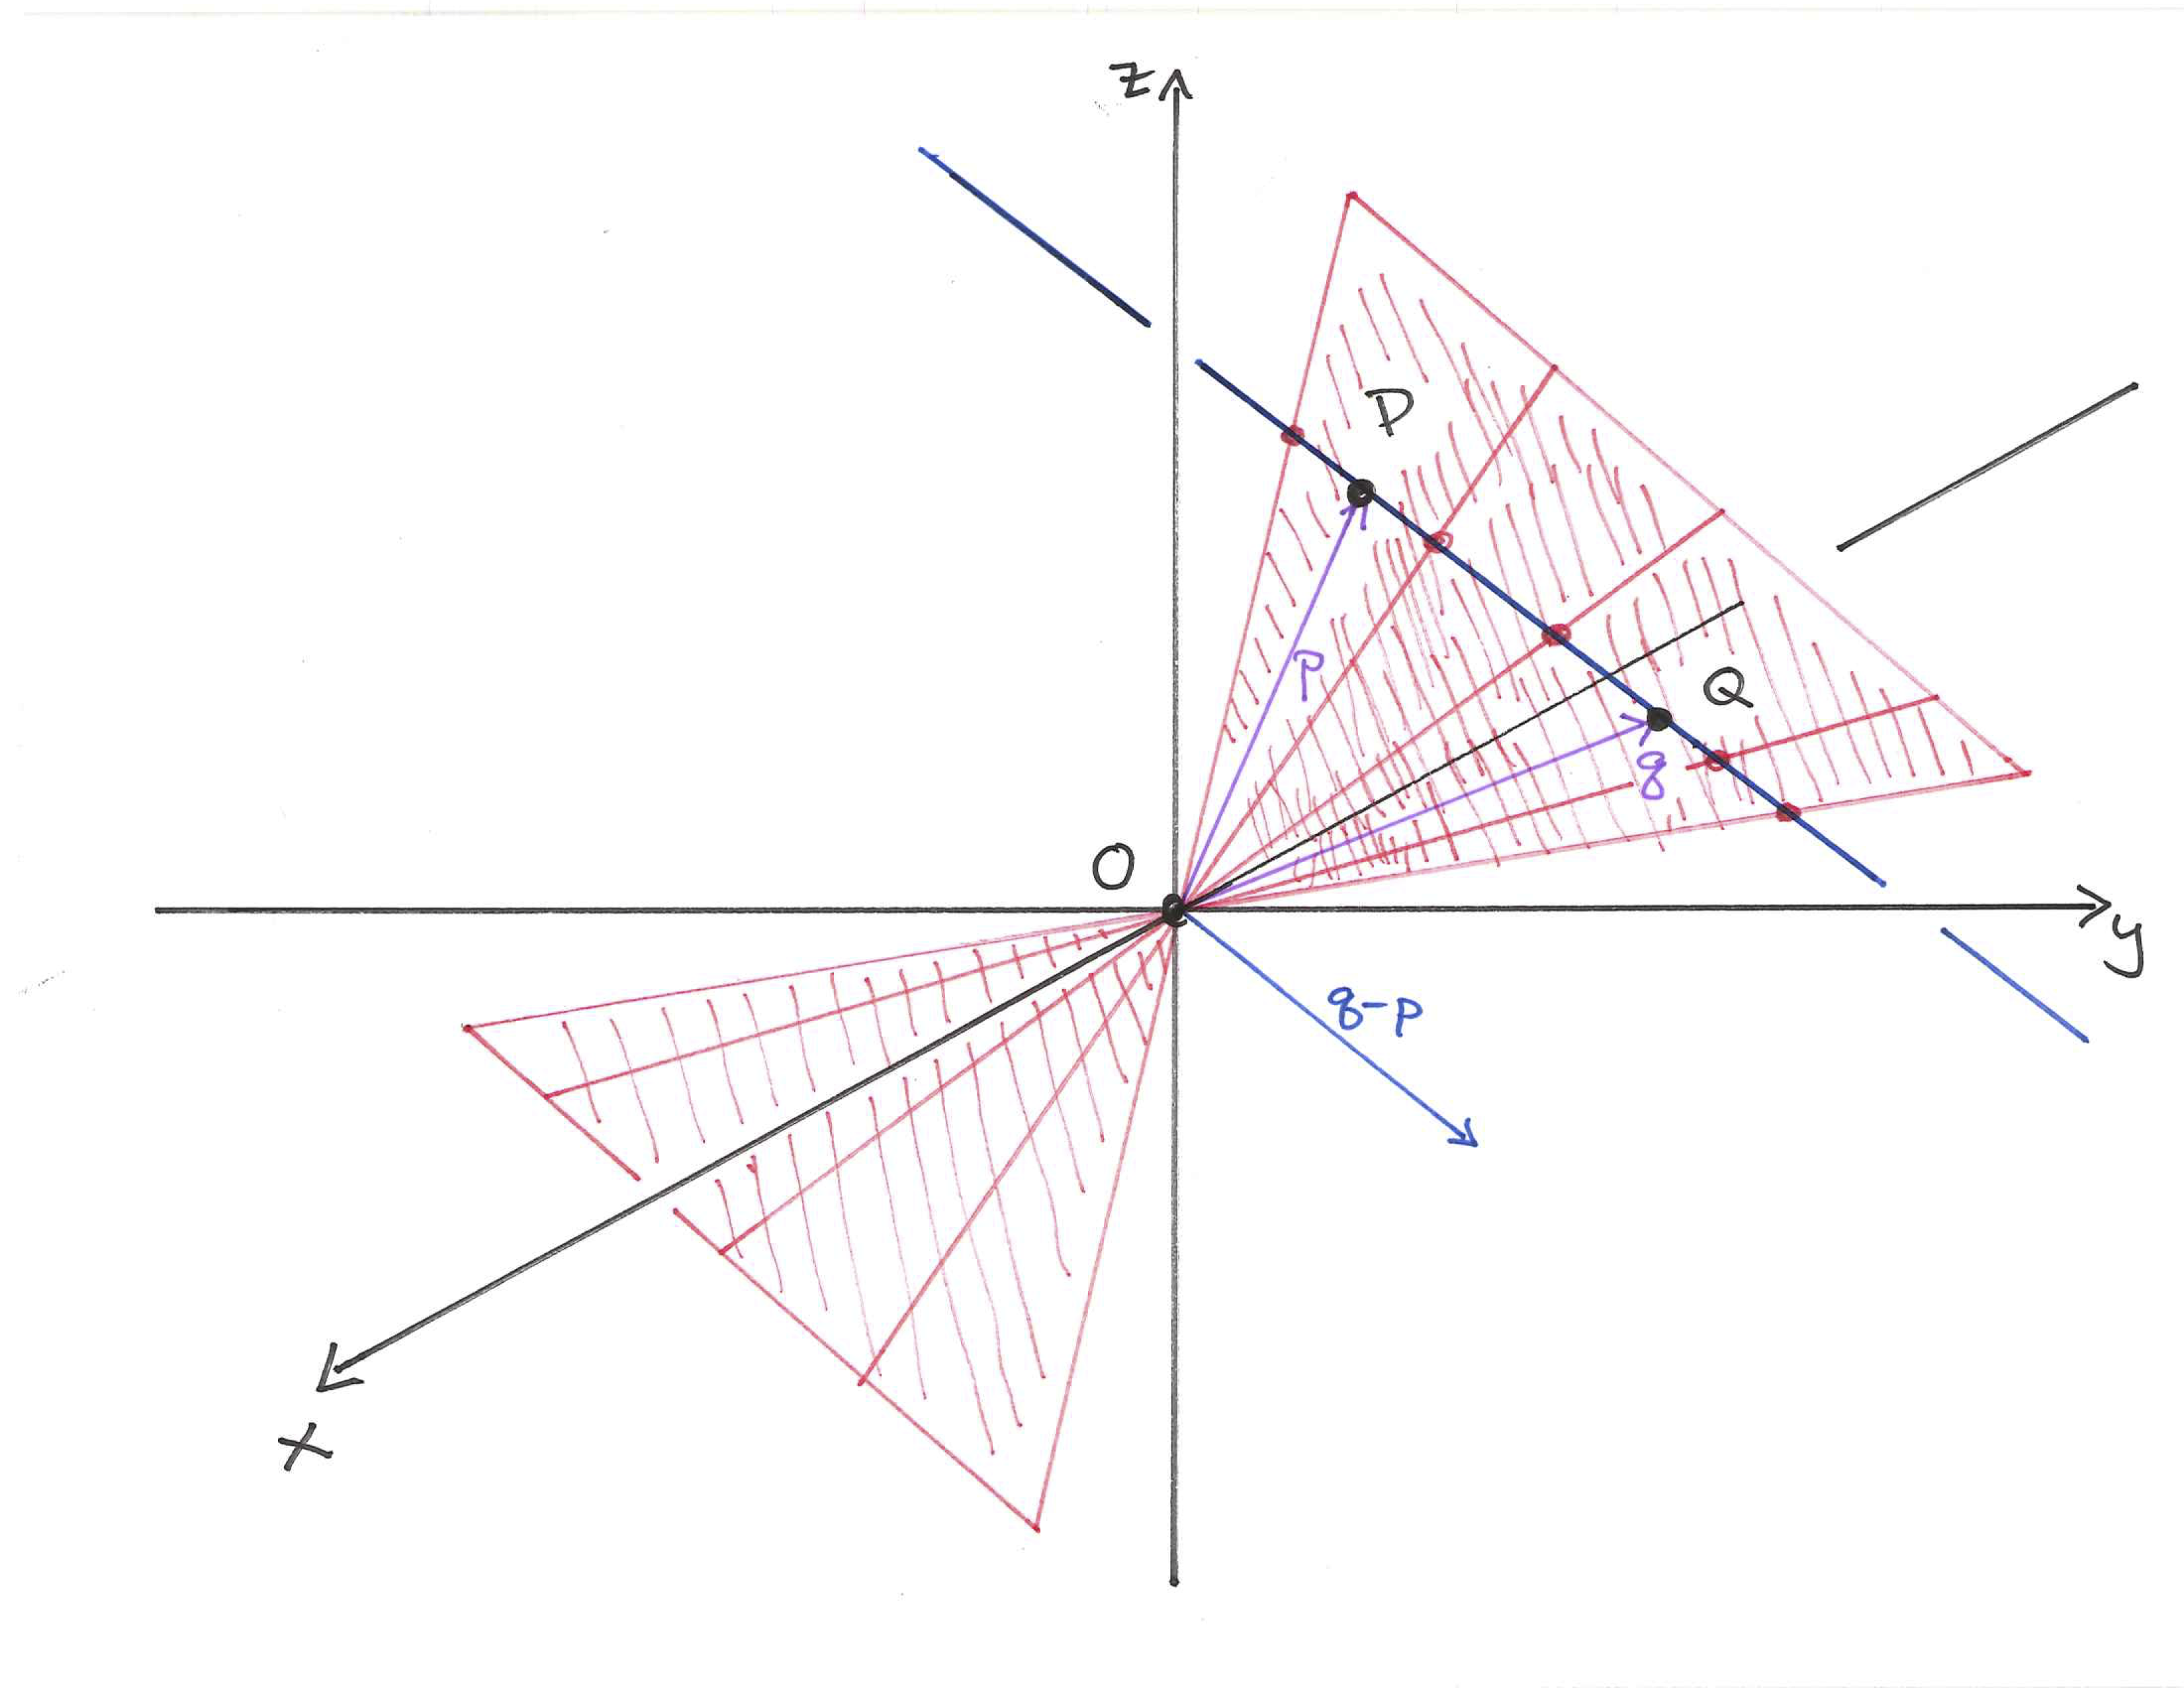
\includegraphics[width=\textwidth]{images/plane-sweep.png}
\caption{The line $PQ$ and the sweep of lines through $O$ and points $X$ on this line.}
\label{fig:parametric-plane-O}
\end{figure}

A careful look at this situation shows that we have described almost all of the points on $\q$. We have missed those on a single line: the line passing through the origin $O$ which is parallel to the line through $P$ and $Q$. That is, our exceptions are the multiples of $q-p$. 

Another way to see this is to look at the two scalars involved in our description, $s(1-t)$ and $st$. There ratio has the form
\[
\frac{st}{s(1-t)} = \frac{t}{1-t}.
\]
But it is not too hard to plot the function $t\mapsto t/(1-t)$ and see that it misses the value $-1$, and only the value $-1$. 

\clearpage
\begin{figure}[h]
\centering
\begin{tikzpicture}[scale=0.8]
\draw[->] (-5,0) -- (5,0) node[below right] {\small $t$};
\draw[->] (0,-3) -- (0,3) node[left] {\small $y$};
\draw[ultra thick, red, domain=3/2:5] plot[smooth] (\x, {\x/(1-\x)});
\draw[ultra thick, red, domain=-5:3/4] plot[smooth] (\x, {\x/(1-\x)});
\draw[dashed] (-5,-1) -- (5,-1);
\draw[thick] (-.1,-1) -- (.1,-1) node [below right] {$y=-1$};
\end{tikzpicture}
\caption{The graph of $y= t/(1-t)$.}
\label{fig:graph-ratio}
\end{figure}

This corresponds to missing vectors of the form $v = \lambda p - \lambda q = \lambda (q-p)$, which is exactly the line through the origin in the direction $q-p$.


Anyway, we can patch the plane back together, and add this line back in, by simply allowing \emph{any} linear combination of the vectors $p$ and $q$.

\begin{theorem}
Let $P$ and $Q$ be two points in $3$-space. If $p$ and $q$ are the vectors with tails at the origin $O$ and heads at $P$ and $Q$, respectively, then the plane through the three points $O$, $P$, and $Q$ is
\[
\q = \left\{ v= s p + t q \middle| \text{$s$ and $t$ are real numbers}\right\}.
\]
\end{theorem}

Now that we have the fact that we can describe a plane through the origin parametrically as the collection of vectors which are linear combinations of two fixed vectors $p$ and $q$, we want to find a way to turn that information into the equation which describes that plane. There are two readily available methods: (1) we can write out some equations and eliminate the parameters $s$ and $t$; or, (2) we can find a normal vector to the plane and use that to write down the equation immediately. These two methods should end up in approximately the same place.

First, let us try the method of eliminating parameters. We will take a variable vector
\[
v = \begin{pmatrix} x \\ y \\z \end{pmatrix}
\]
which we assume to lie in our plane $\q$. Our goal is to find an equation satisfied by $x$, $y$, and $z$. In order to make progress, we will need to have more detailed notation for $p$ and $q$, so we write them out in coordinates as
\[
p = \begin{pmatrix} p_1 \\ p_2 \\ p_3 \end{pmatrix} \quad \text{ and } \quad
q = \begin{pmatrix} q_1 \\ q_2 \\ q_3 \end{pmatrix} .
\]



Since $v$ is in $\q$, we can write
\[
\begin{pmatrix} x \\ y \\ z \end{pmatrix} = s \begin{pmatrix} p_1 \\ p_2 \\ p_3 \end{pmatrix} + t \begin{pmatrix} q_1 \\ q_2 \\ q_3 \end{pmatrix}.
\]
We then unbundle this vector equation into three separate equations, one for each coordinate.\footnote{We are about to do a computation involving $11$ different variables. This looks intimidating, but it isn't so bad. Just stay calm and do it. Choose a particular example and follow along by doing the steps for yourself.}
\[
\left\{ \begin{array}{rrrrr}
x & = & p_1 s & + & q_1 t \\
y & = & p_2 s & + & q_2 t \\
z & = & p_3 s & + & q_3 t 
\end{array}\right.
\]

Our first step is to eliminate $s$ using the first two equations. We do this by multiplying the first equation by $p_2$ and the second by $-p_1$ and then adding.
We obtain
\[
p_2 x - p_1 y = t (p_2q_1 - p_1 q_2).
\]
Similarly, we will eliminate $s$ by using the second and third equations. We do this by multiplying the second equation by $p_3$ and the third by $-p_2$ and then adding. We obtain
\[
p_3 y - p_2 z = t (p_3 q_2 - p_2 q_3).
\]
This gives us a pair of equations relating $x$, $y$, and $z$ to $t$. We have effectively eliminated $s$. So, now consider our new system of equations:
\[
\left\{ \begin{array}{rrrrr}
p_2 x &-& p_1 y &=& t (p_2q_1 - p_1 q_2) \\
p_3 y &-& p_2 z &=& t (p_3 q_2 - p_2 q_3)
\end{array}\right.
\]
It remains to eliminate $t$ from these. The clearest way to do that is to multiply the first equation by $p_3q_2-p_2q_3$ and the second equation by $-(p_2q_1 - p_1 q_2)$ and then add. We do this to find
\[
(p_3 q_2 - p_2 q_3)(p_2 x - p_1 y) -(p_2q_1 - p_1 q_2)(p_3 y - p_2 z) = 0.
\]
This is our equation! All of the $s$'s and $t$'s are gone, and we are done.
Now, in practice, it is better to have things organized so that like terms are together. If we do a little bit of manipulation and cleaning up, we eventually get this:
\[
\left\{p_2(p_3 q_2 - p_2 q_3)\right\} x +
\left\{p_2(p_1 q_3 - p_3 q_1)\right\} y +
\left\{p_2(p_2 q_1 - p_1 q_2)\right\} z = 0.
\]
Note that there is a $p_2$ multiplied through the whole thing, so we should factor it out and get rid of it. That leaves us with
\[
(p_3 q_2 - p_2 q_3) x +
(p_1 q_3 - p_3 q_1) y +
(p_2 q_1 - p_1 q_2) z = 0.
\]
This is the equation of our plane $\q$, written in a relatively convenient form.
We can read off of this expression that a normal vector to $\q$ is 
\[
n = \begin{pmatrix} p_3 q_2 - p_2 q_3 \\
p_1 q_3 - p_3 q_1 \\ p_2 q_1 - p_1 q_2 \end{pmatrix}.
\]



Now let us try the other method. We know that $\q$ is the collection of linear combinations of $p$ and $q$, and the normal vector to $\q$ must be orthogonal to every one of those vectors. In particular, the normal vector has to be orthogonal to $p$ and to $q$. We keep the same notation for components of $p$ and $q$ as above, and introduce notation for $n$ as follows:\footnote{We are about to do a computation involving $9$ different variables. This looks intimidating, but it isn't so bad. Just stay calm and do it. Choose a particular example and follow along by doing the steps for yourself.}
\[
n = \begin{pmatrix} n_1 \\ n_2 \\ n_3 \end{pmatrix} .
\]
The fact that $n$ is orthogonal to both $p$ and $q$ leads us to this pair of equations
\[
\left\{ \begin{array}{rrrrrrr}
p_1 n_1 & + & p_2 n_2 & + & p_3 n_3 & = & 0 \\
q_1 n_1 & + & q_2 n_2 & + & q_3 n_3 & = & 0 
\end{array}\right. .
\]
We have to do a similar sort of elimination process here to figure out what the $n_i$'s are in terms of the other variables. We are going to do this in a slightly different fashion than the above. It will feel less symmetrical than what we have done before, but it will be very efficient.

Our first step is to multiply the first equation through by $-q_1/p_1$ and then add it to the second equation. Then we'll take a look at our updated system.
\[
\left\{ \begin{array}{rrrrrrr}
p_1 n_1 & + & p_2 n_2 & + & p_3 n_3 & = & 0 \\
& &\left(q_2-\frac{p_2q_1}{p_1}\right) n_2 & + & \left(q_3-\frac{p_3q_1}{p_1}\right) n_3 & = & 0 
\end{array}\right. .
\]
Next, we will multiply the second equation by the number 
\[
\frac{-p_2}{q_2 - \frac{p_2q_1}{p_1}} = \frac{-p_1p_2}{p_1q_2 - p_2q_1}
\] 
and add the result back into the first equation. After a lots of work with fractions, we see that this updates our system to read
\[
\left\{ \begin{array}{rrrrrrr}
p_1 n_1 &  &  & + & \left(p_3 -\frac{p_1q_3-p_3q_1}{p_1q_2 - p_2q_1}p_2  \right) n_3 & = & 0 \\
& &\left(q_2-\frac{p_2q_1}{p_1}\right) n_2 & + & \left(q_3-\frac{p_3q_1}{p_1}\right) n_3 & = & 0 
\end{array}\right. .
\]
We are certainly not happy with this, yet. To clean up some more, we can work out that $n_3$ term in the first equation. Then we obtain
\[
\left\{ \begin{array}{rrrrrrr}
p_1 n_1 &  &  & + & p_1\frac{p_3q_2 - p_2q_3}{p_1q_2-p_2q_1} n_3 & = & 0 \\
& &\left(q_2-\frac{p_2q_1}{p_1}\right) n_2 & + & \left(q_3-\frac{p_3q_1}{p_1}\right) n_3 & = & 0
\end{array}\right. .
\]
Finally, divide through the second equation by the coefficient of $n_2$, and divide through the first equation by $p_1$ to get rid of a common factor. We now have something that does not look overly scary.
\[
\left\{ \begin{array}{rrrrrrr}
n_1 &  &  & + & \frac{p_3q_2 - p_2q_3}{p_1q_2-p_2q_1} n_3 & = & 0 \\
& & n_2 & + & \frac{p_1q_3-p_3q_1}{p_1q_2-p_2q_1} n_3 & = & 0 
\end{array}\right. .
\]



Something wonderful has happened. Note that in each equation, only two of the variables $n_i$ appear. In fact, if we just choose $n_3$, then the equations tell us exactly what $n_1$ and $n_2$ should be. We can just write
\[
n = \begin{pmatrix}  \frac{p_2q_3 - p_3q_2}{p_1q_2-p_2q_1} n_3\\ \frac{p_3q_1-p_1q_3}{p_1q_2-p_2q_1} n_3\\ n_3 \end{pmatrix} = n_3 \begin{pmatrix}  \frac{p_2q_3 - p_3q_2}{p_1q_2-p_2q_1} \\ \frac{p_3q_1-p_1q_3}{p_1q_2-p_2q_1} \\ 1 \end{pmatrix}
\]


This is a good sign. Recall that a plane has many normal vectors. If we find one, we could always just rescale it to get another one. Since our work shows us this property, we should be happy. 

But for now, we just want to find any one single normal vector, so we have to make a choice. And it would be good to make a choice that helps simplify all of the messy fractions we have derived. We choose $n_3 = p_1q_2 - p_2q_1$ so that we can easily clear the denominator common to the first two coordinates. We substitute this expression in, and we have finally found that our preferred normal vector\footnote{Some texts call this particular choice of $n$ the \emph{cross product} of $p$ and $q$.} is
\[
n = \begin{pmatrix} p_2 q_3 - p_3 q_2 \\
p_3 q_1 - p_1 q_3 \\ p_1 q_2 - p_2 q_1 \end{pmatrix}.
\]
We deduce that the equation for the plane must be
\[
0 = \begin{pmatrix}x \\ y \\ z \end{pmatrix} \cdot \begin{pmatrix} p_2 q_3 - p_3 q_2 \\
p_3 q_1 - p_1 q_3 \\ p_1 q_2 - p_2 q_1 \end{pmatrix},
\]
or, more simply, 
\[
(p_2 q_3 - p_3 q_2) x +
(p_3 q_1 - p_1 q_3) y +
(p_1 q_2 - p_2 q_1) z = 0.
\]
This is our desired result.

We should compare our two versions of the work. Looking carefully, we see that the only differences in the end results are of sign. The normal vectors are the same, up to multiplying by the scalar $-1$, and the equations are the same up to multiplying through by $-1$.

After all of that intense computation, it feels like a little bit of a miracle. But the miracle is just that we did things carefully and got through without arithmetic errors.

\begin{theorem}\label{thm:plane-2-points}
Let $\q$ be a plane in $\R^3$ which passes through the origin $O$ and two points $P = (p_1,p_2,p_3)$ and $Q=(q_1,q_2,q_3)$. Then any normal vector to $\q$ is a scalar multiple of the vector
\[
n = \begin{pmatrix} p_2 q_3 - p_3 q_2 \\
p_3 q_1 - p_1 q_3 \\ p_1 q_2 - p_2 q_1 \end{pmatrix},
\]
and the plane may be described as the set of points which satisfy the equation
\[
(p_2 q_3 - p_3 q_2) x +
(p_3 q_1 - p_1 q_3) y +
(p_1 q_2 - p_2 q_1) z = 0,
\]
or parametrically as the image of 
\[
(s,t) \mapsto s \begin{pmatrix} p_1 \\ p_2 \\ p_3 \end{pmatrix} + t \begin{pmatrix} q_1 \\ q_2 \\ q_3 \end{pmatrix}.
\]
\end{theorem}

\section*{General Planes in $\R^3$}

So far, all of our hard work has led us to a deep understanding of planes in $\R^3$, but only those that pass through the origin $O$. But most of the planes in $\R^3$ do not contain the origin. We must figure out how to handle those, too.

In the case of lines in the plane, we used a simple method: Given a line not through the origin, find a parallel line through the origin. Describe that line by whatever method you want, and then translate back to get the description you want. We shall use this same method here. 

\begin{definition}
Let $\p$ and $\q$ be planes in $\R^3$. We say that $\p$ and $\q$ are \emph{parallel} if they have no points in common.
\end{definition}

So, we begin with three points which define a plane $\p$ in $\R^3$. Call them $P$, $Q$, and $R$. As usual, we write $p$, $q$, and $r$ for the mathematician's vectors which have their heads at these three points, respectively. Now the physicist's vectors $p-r$ and $q-r$ lie entirely in in $\p$. The corresponding mathematician's vectors lie in a plane $\q$ which is parallel to $\p$. Also, the new plane $\q$ contains the origin. In fact, these two planes differ exactly by a parallel translation by the vector $r$: for each vector $v$ with its head in $\p$, the corresponding vector $v-r$ lies entirely in $\q$.

Now, since the plane $\q$ passes through the origin, we can give it one of our two types of descriptions, each of which will help us build the corresponding description for the plane $\p$. Let us take them in turn, starting with the
parametric description. 


The plane $\q$ is the collection of vectors formed by linear combinations of $p-r$ and $q-r$.
\[
s (p-r) + t (q-r).
\] 
Since $v-r$ lies in $\q$, we see that
\[
v-r = s(p-r) + t (q-r),
\]
or 
\[
v = r + s(p-r) + t (q-r).
\]
Since each of the vectors $p$, $q$, and $r$ are known to us, it is straightforward to compute this explicitly. We get the parametric description
\[
(s,t) \mapsto r + s(p-r) + t (q-r)
\]



Next, let us consider the equation of $\p$.
The plane $\q$ is the set of points $w=(x,y,z)$ which are orthogonal to the normal vector $n$ which is as described in Theorem \ref{thm:plane-2-points}.
But $v-r$ is an element of $\q$, so we see that our equation for $\p$ is just
\[
n \cdot (v-r) = 0, \quad \text{or} \quad n\cdot v = n \cdot r.
\]
The trick is that first you must compute $n$ from $p-r$ and $q-r$. If $n$ has components $a$, $b$, and $c$, we get an equation of the form 
\[
ax+by+cz = d.
\]
Since the planes $\p$ and $\q$ are parallel, they share the same normal vector. This is apparent in the structure of their equations: the coefficients of the variables represent the normal vector, and they are the same. But the number on the right-hand side, $d$, depends on exactly which plane you consider in the family of parallel planes with normal vector $n$.

If we put together all of this work with the things we learned above, we obtain this result.

\begin{theorem}
Let $\p$ be the plane in $\R^3$ which contains the points $R = (r_1, r_2, r_3)$, $P=(p_1,p_2,p_3)$, and $Q=(q_1,q_2,q_3)$. Let $p$, $q$, and $r$ be the vectors with their heads at these points, respectively. Then we have the following:
\begin{itemize}
\item $\p$ is parallel to a plane $\q$ which passes through the origin. These two planes have a common normal vector
\[
n = \begin{pmatrix} a \\ b \\ c \end{pmatrix} := 
\begin{pmatrix} (p_2-r_2)( q_3-r_3) - (p_3 -r_3)(q_2-r_2) \\
(p_3-r_3)(q_1-r_1) - (p_1-r_1)( q_3-r_3) \\ (p_1-r_1)(q_2-r_2) - (p_2-r_2) (q_1-r_1) \end{pmatrix}
\]

\item $\p$ has the parametric description
\[
(s,t) \mapsto r + s (p-r) + t(q-r).
\]

\item $\p$ has the equation
\[
ax + by +cz = ar_1 + br_2 + cr_3,
\]
where $a, b, c$ are the components of $n$ as above.
\end{itemize}
\end{theorem}

It is worth noting that the actual techniques of our earlier work carry over just fine, too. We can pass back and forth between a parametric description of a plane and an equation for that plane.

Suppose you have the equation $ax+by+cz = d$. To find a parametric description of the plane, do the following.
\begin{enumerate}
\item Choose a nonzero coefficient. For simplicity, assume it is $a\neq 0$. Then solve 
for the corresponding variable:
\[
x  = \frac{d}{a} - \frac{b}{a} y - \frac{c}{a} z.
\]

\item Choose parameter names, and introduce dummy equations for them. Say $y=s$ and $z=t$.

\item Substitute the new parameters in the equation, and set up a system of all of the equations you have:
\[
\left\{ \begin{array}{rrrrrrr}
x  &=& \frac{d}{a} &-& \frac{b}{a} s &-& \frac{c}{a} t \\
y  &=&             & &             s & &  \\
y  &=&             & &               & & t 
\end{array}\right. .
\]

\item Rewrite the system as a vector equation.
\[
\begin{pmatrix} x \\ y \\ z \end{pmatrix} = 
\begin{pmatrix} \frac{d}{a} \\ 0 \\ 0 \end{pmatrix} + 
s\begin{pmatrix} -\frac{b}{a} \\ 1 \\ 0 \end{pmatrix} +
t\begin{pmatrix} -\frac{c}{a} \\ 0 \\ 1 \end{pmatrix} .
\]
\end{enumerate}

In the other direction, suppose that you have a parametric description and want to change it into an equation. The key is to unbundle the parametric description into a system of equations, and then steadily eliminate the variables.

If the system of equations is
\[
\left\{ \begin{array}{rrrrrrr}
x  &=& a &+& b s &+& c t \\
y  &=& d &+& e s &+& f t \\
z  &=& g &+& h s &+& i t 
\end{array}\right. ,
\]
Then we can use the first and second equation to eliminate $s$, and then the second and third equations to also eliminate $s$, to get two equations involving only $x,y,z,$ and $t$, like so:\footnote{I ran out of symbols, so here are some new friends. The letters $\alpha, \beta, \gamma, \delta$ come from an old form of Greek, and are called alpha, beta, gamma, and delta.}
\[
\left\{ \begin{array}{rrrrr}
ex-by &=& \alpha &+& \beta t \\
gy-ez &=& \gamma &+& \delta t
\end{array}\right. ,
\]
Now we can similarly use these two equations to eliminate $t$ and obtain an equation of the form
\[
Ax+By+Cz = D.
\]


\section*{Lines in $\R^3$ as Solutions to Systems of Equations}

We had a major goal to describe lines in $\R^3$, but got distracted by the nature of planes in $3$-space.

So, how can we find something like an equation for a line in $\R^3$? We have learned that a single equation relating three variables $x$, $y$, and $z$ ends up describing a plane. This means that a single equation can't work!

The key idea is that a line what you get when you intersect two planes. So, to describe a line, we need two equations, not one.

Suppose we are given a line described parametrically. $t \mapsto p + tv$.
How can we find two equations which will together describe the line? Well, our line has a direction vector $v$. Choose two vectors $n_{\p}$ and $n_{\q}$ which are orthogonal to $v$ and are not scalar multiples of each other. There are lots and lots of pairs of vectors like this, just pick. It seems like a staggering amount of freedom, but we might as well enjoy it.

Now we consider the plane $\p$ with equation
\[
n_{\p} \cdot  \begin{pmatrix} x \\ y \\ z \end{pmatrix}  = n_{\p}\cdot p ,
\]
and the plane $\q$ with equation
\[
n_{\q} \cdot  \begin{pmatrix} x \\ y \\ z \end{pmatrix}  = n_{\q}\cdot p .
\]
Since the normal vectors $n_{\p}$ and $n_{\q}$ are not scalar multiples of each other, these planes are not parallel. That means these planes intersect along a line. The important thing is that the line of intersection is exactly our line. To see this, we just check that the vectors $p+t v$ satisfy the two equations. It is straightforward to check this directly:
\[
n_{\p} \cdot (p + tv) = n_{\p} \cdot p + t n_{\p}\cdot v = n_{\p}\cdot p + 0 = n_{\p}\cdot p,
\]
so the vectors $p+tv$ have heads in $\p$, and 
\[
n_{\q} \cdot (p + tv) = n_{\q} \cdot p + t n_{\q}\cdot v = n_{\q}\cdot p + 0 = n_{\q}\cdot p,
\]
so the vectors $p+tv$ also have heads in $\q$.

\begin{theorem}
A line in $\R^3$ can be described as the common solution set for a system of equations representing two planes
\[
\left\{\begin{array}{rrrrrrr}
a_{11} x &+& a_{12}y &+& a_{13} z &=& b_1 \\
a_{21} x &+& a_{22}y &+& a_{23} z &=& b_2 \\
\end{array}\right.
\]
Where the two normal vectors
\[
n_1 = \begin{pmatrix} a_{11} \\ a_{12} \\ a_{13} \end{pmatrix}, \quad \text{and} \quad
n_2 = \begin{pmatrix} a_{21} \\ a_{22} \\ a_{23} \end{pmatrix}
\]
are both orthogonal to the direction vector $v$ of the line, but are not scalar multiples of each other.

There are many such pairs of planes which have the line as their intersection.
\end{theorem}


This shows us how we might go from a parametric description to a system of equations. How might we work in the other direction? Suppose we are given a pair of planes described by equations, and we wish to find a parametric description for the line which is their common solution set.

Now the process is exactly that like we used to find a normal vector to a plane through the origin. Just as in the few pages running up to Theorem \ref{thm:plane-2-points}, we have a pair of equations and we want a common solution. The idea is to replace the very general set of equations 
\[
\left\{\begin{array}{rrrrrrr}
a_{11} x &+& a_{12}y &+& a_{13} z &=& b_1 \\
a_{21} x &+& a_{22}y &+& a_{23} z &=& b_2 \\
\end{array}\right.
\]
with a nicer, equivalent set of equations that looks like this
\[
\left\{\begin{array}{rrrrrrr}
x &&  &+& \alpha z &=& d_1 \\
 && y &+& \beta z &=& d_2 \\
\end{array}\right. ,
\]
which we can rewrite in vector form as the parametric description
\[
\begin{pmatrix} x \\ y \\ z \end{pmatrix} = 
\begin{pmatrix} d_1 \\ d_2 \\ 0 \end{pmatrix} + 
t \begin{pmatrix} -\alpha \\ -\beta \\ 1 \end{pmatrix} .
\]

This process is routine to do once learned, but it doesn't always work. There are two kinds of trouble that could happen. 

The first is that some pairs of equations represent planes that actually don't intersect. The planes are parallel, and at some point we find an equation that doesn't actually make any sense, like $0=1$.

The second problem is that some pairs of equations are really the same plane written twice. In this case, the solution set is all of (both of) the planes, not a line. Then the process ends up turning one equation into something trivially true, usually $0=0$, and the rest collapses back on our technique for writing the parametric description for the plane.

Both of these situations require that the normal vectors to the planes are scalar multiples of each other, so with a little bit of care, you can learn to look for that before getting started on the time-consuming arithmetic.

\begin{theorem}
There are three cases possible for the shape of the set of simultaneous solutions to a system of 2 equations in three unknowns.
\begin{description}
\item[Generic Case:] The two equations represent a pair of planes which are not parallel. The solution set is a line in $\R^3$.
\item[Degenerate Case 1:] The two equations are different representations for the same plane. The solution set is that plane.
\item[Degenerate Case 2:] The two equations represent planes which are distinct, but parallel. There are no solutions because the planes do not intersect.
\end{description}
\end{theorem}

\end{document}